% poster.tex -- ISU Honors Poster Symposium
% AS-TWAS-COLOC: Colocalization-Confirmed TWAS of Ankylosing Spondylitis
% 48" x 36" landscape, beamerposter
% Build: latexmk -pdf poster.tex  (or: make poster)

\documentclass[final]{beamer}
\usepackage[orientation=landscape, size=custom, width=121.92, height=91.44, scale=1.0]{beamerposter}
\usepackage{beamerthemeISU}
\usepackage[T1]{fontenc}
\usepackage{lmodern}
\usepackage{amsmath, amssymb}
\usepackage{graphicx}
\usepackage{booktabs}
\usepackage{tikz}
\usetikzlibrary{shapes.geometric, arrows.meta, positioning, fit, backgrounds, calc}
\usepackage{multicol}
\usepackage{ragged2e}
\usepackage{qrcode}
\usepackage{caption}
\captionsetup{font=small, labelfont=bf, labelsep=period, skip=0.35em}

% ── Metadata ─────────────────────────────────────────────────────────────────
\title{Colocalization-Confirmed Transcriptome-Wide Association Study\\
of Ankylosing Spondylitis to Prioritize Tissue-Specific Drug Targets}
\author{Bhargav Yellepeddi \quad $\cdot$ \quad Advisor: Dr.\ Ratul Chowdhury}
\date{}

% ── Document ─────────────────────────────────────────────────────────────────
\setlength{\belowcaptionskip}{0.25em}
\setlength{\columnsep}{1.2cm}
\begin{document}
\begin{frame}[t]
\begin{columns}[t,onlytextwidth]

% ══════════════════════════════════════════════════════════════════════════════
% COLUMN 1 (left): Introduction, Key Question, Methods, Conclusion, Future
% ══════════════════════════════════════════════════════════════════════════════
\begin{column}{0.32\textwidth}

% ── Introduction ─────────────────────────────────────────────────────────────
\begin{block}{Introduction}
\justifying
\textbf{Ankylosing spondylitis (AS)} is a chronic inflammatory arthritis of
the spine and sacroiliac joints affecting 0.1--0.5\% of the population,
with onset typically before age~30. GWAS have identified over 100 risk loci,
but most fall in non-coding regions.

\vskip0.4em
\textbf{Transcriptome-wide association studies (TWAS)} integrate GWAS with
gene expression models to identify genes whose genetically regulated
expression is associated with disease. However, TWAS hits can arise from
\textit{linkage disequilibrium (LD) contamination} rather than true shared
causal variants.

\vskip0.4em
\textbf{Bayesian colocalization} tests whether a GWAS signal and an eQTL
signal share the same causal variant, filtering LD artifacts.
\end{block}

% ── Key Question ─────────────────────────────────────────────────────────────
\begin{alertblock}{Key Question}
\centering\large
Which genes have genetically regulated expression that \textbf{causally
colocalizes} with AS risk variants, and in which tissues?
\end{alertblock}

% ── Methods ──────────────────────────────────────────────────────────────────
\begin{block}{Methods}
\justifying

% Methods flowchart
\begin{center}
\begin{tikzpicture}[
  node distance=0.5cm and 0.4cm,
  box/.style={rectangle, rounded corners=3pt, draw=ISURed, fill=ISURed!8,
              text width=14em, minimum height=2em, align=center,
              font=\footnotesize\bfseries},
  data/.style={rectangle, rounded corners=3pt, draw=ISUGold, fill=ISUGold!15,
               text width=12em, minimum height=1.8em, align=center,
               font=\footnotesize},
  arrow/.style={-{Stealth[length=2.5mm]}, thick, ISUDark}
]
  \node[data] (gwas) {AS GWAS (GCST005529)\\$N$=25,764};
  \node[data, right=1.2cm of gwas] (gtex) {GTEx v8 Mashr Models\\8 tissues};
  \node[box, below=0.4cm of $(gwas)!0.5!(gtex)$] (harm) {1. GWAS QC \& Harmonization};
  \node[box, below=of harm] (twas) {2. S-PrediXcan TWAS};
  \node[box, below=of twas] (fdr) {3. FDR Correction (BH, $\alpha$=0.05)};
  \node[box, below=of fdr] (coloc) {4. Colocalization (PP4 $\geq$ 0.70)};
  \node[box, below=of coloc] (out) {5. Prioritized Gene List};

  \draw[arrow] (gwas.south) -- ++(0,-0.2) -| (harm.north);
  \draw[arrow] (gtex.south) -- ++(0,-0.2) -| (harm.north);
  \draw[arrow] (harm) -- (twas);
  \draw[arrow] (twas) -- (fdr);
  \draw[arrow] (fdr) -- (coloc);
  \draw[arrow] (coloc) -- (out);
\end{tikzpicture}
\end{center}

\textbf{GWAS QC:} 123,941 SNPs $\to$ liftOver hg38 $\to$ 14,032
palindromic removed $\to$ 109,893 harmonized.

\vskip0.2em
\textbf{Tissues:} Whole Blood, Spleen, Lung, Colon Sigmoid, Colon
Transverse, Small Intestine, Muscle Skeletal, Adipose Subcutaneous.
\end{block}

% ── Conclusion ───────────────────────────────────────────────────────────────
\begin{block}{Conclusion}
\justifying
Integrating S-PrediXcan TWAS with Bayesian colocalization identified
\textbf{18 unique genes} with shared causal variants at AS risk loci,
prioritizing tissue-specific targets for therapeutic development.
\end{block}

% ── Future Directions ────────────────────────────────────────────────────────
\begin{alertblock}{Future Directions}
\begin{itemize}\setlength{\itemsep}{1pt}
  \item Fine-mapping with SuSiE for credible causal variants
  \item Validation in independent AS cohorts
  \item Drug repurposing analysis for top targets
\end{itemize}
\end{alertblock}

\end{column}

% ══════════════════════════════════════════════════════════════════════════════
% COLUMN 2 (center): TWAS Results, Colocalization Results, Discussion
% ══════════════════════════════════════════════════════════════════════════════
\begin{column}{0.34\textwidth}

% ── TWAS Results ─────────────────────────────────────────────────────────────
\begin{block}{TWAS Results}
\justifying
S-PrediXcan tested \textbf{2,316 gene-tissue pairs} across 8 GTEx v8
tissues. After Benjamini--Hochberg FDR correction ($\alpha = 0.05$),
\textbf{248 significant associations} were identified, spanning genes on
multiple chromosomes.

\vskip0.3em
\begin{center}
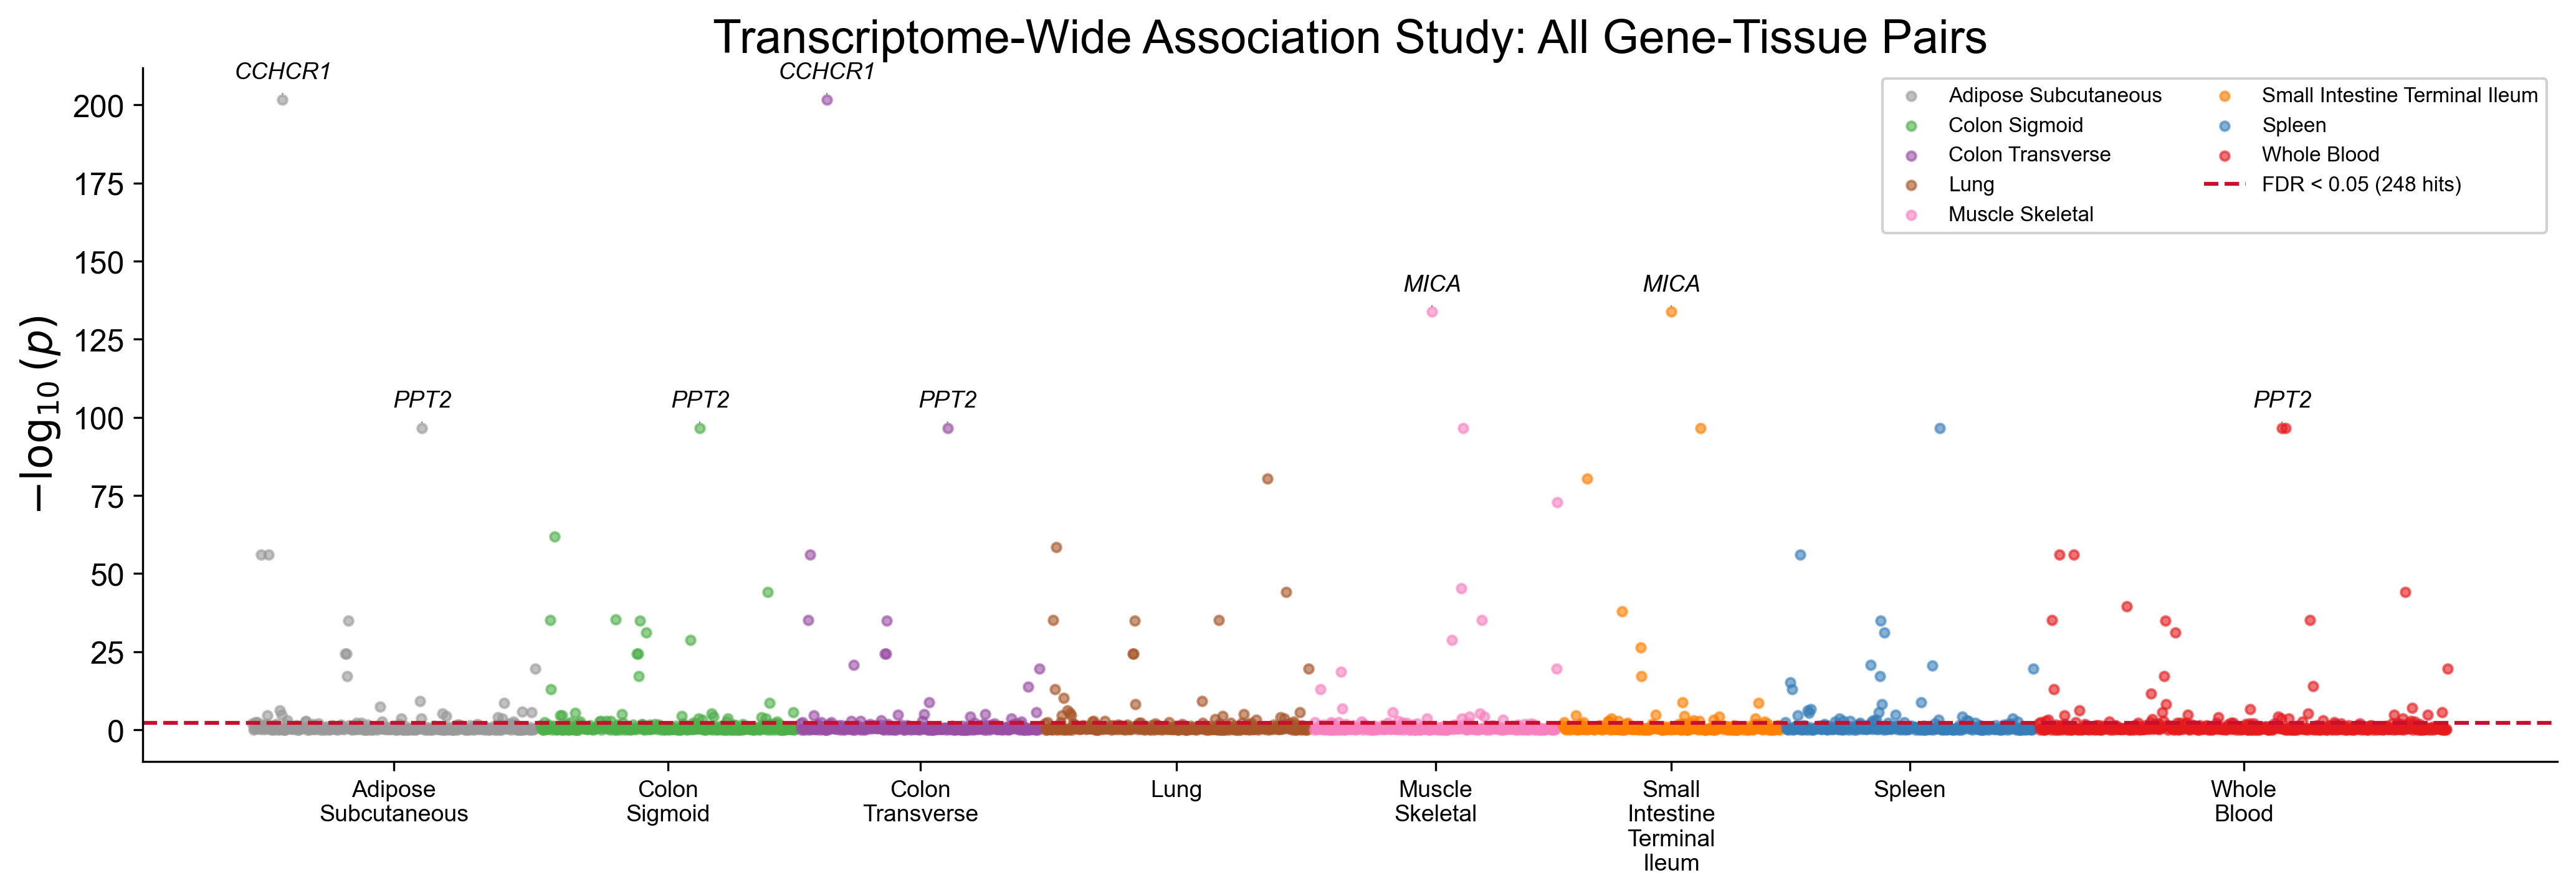
\includegraphics[width=0.92\linewidth]{figures/manhattan_twas.png}
\captionof{figure}{Manhattan-style plot of TWAS $-\!\log_{10}(p)$ across 8
tissues. Top gene symbols annotated. Dashed line: FDR $< 0.05$.}
\end{center}

\begin{center}
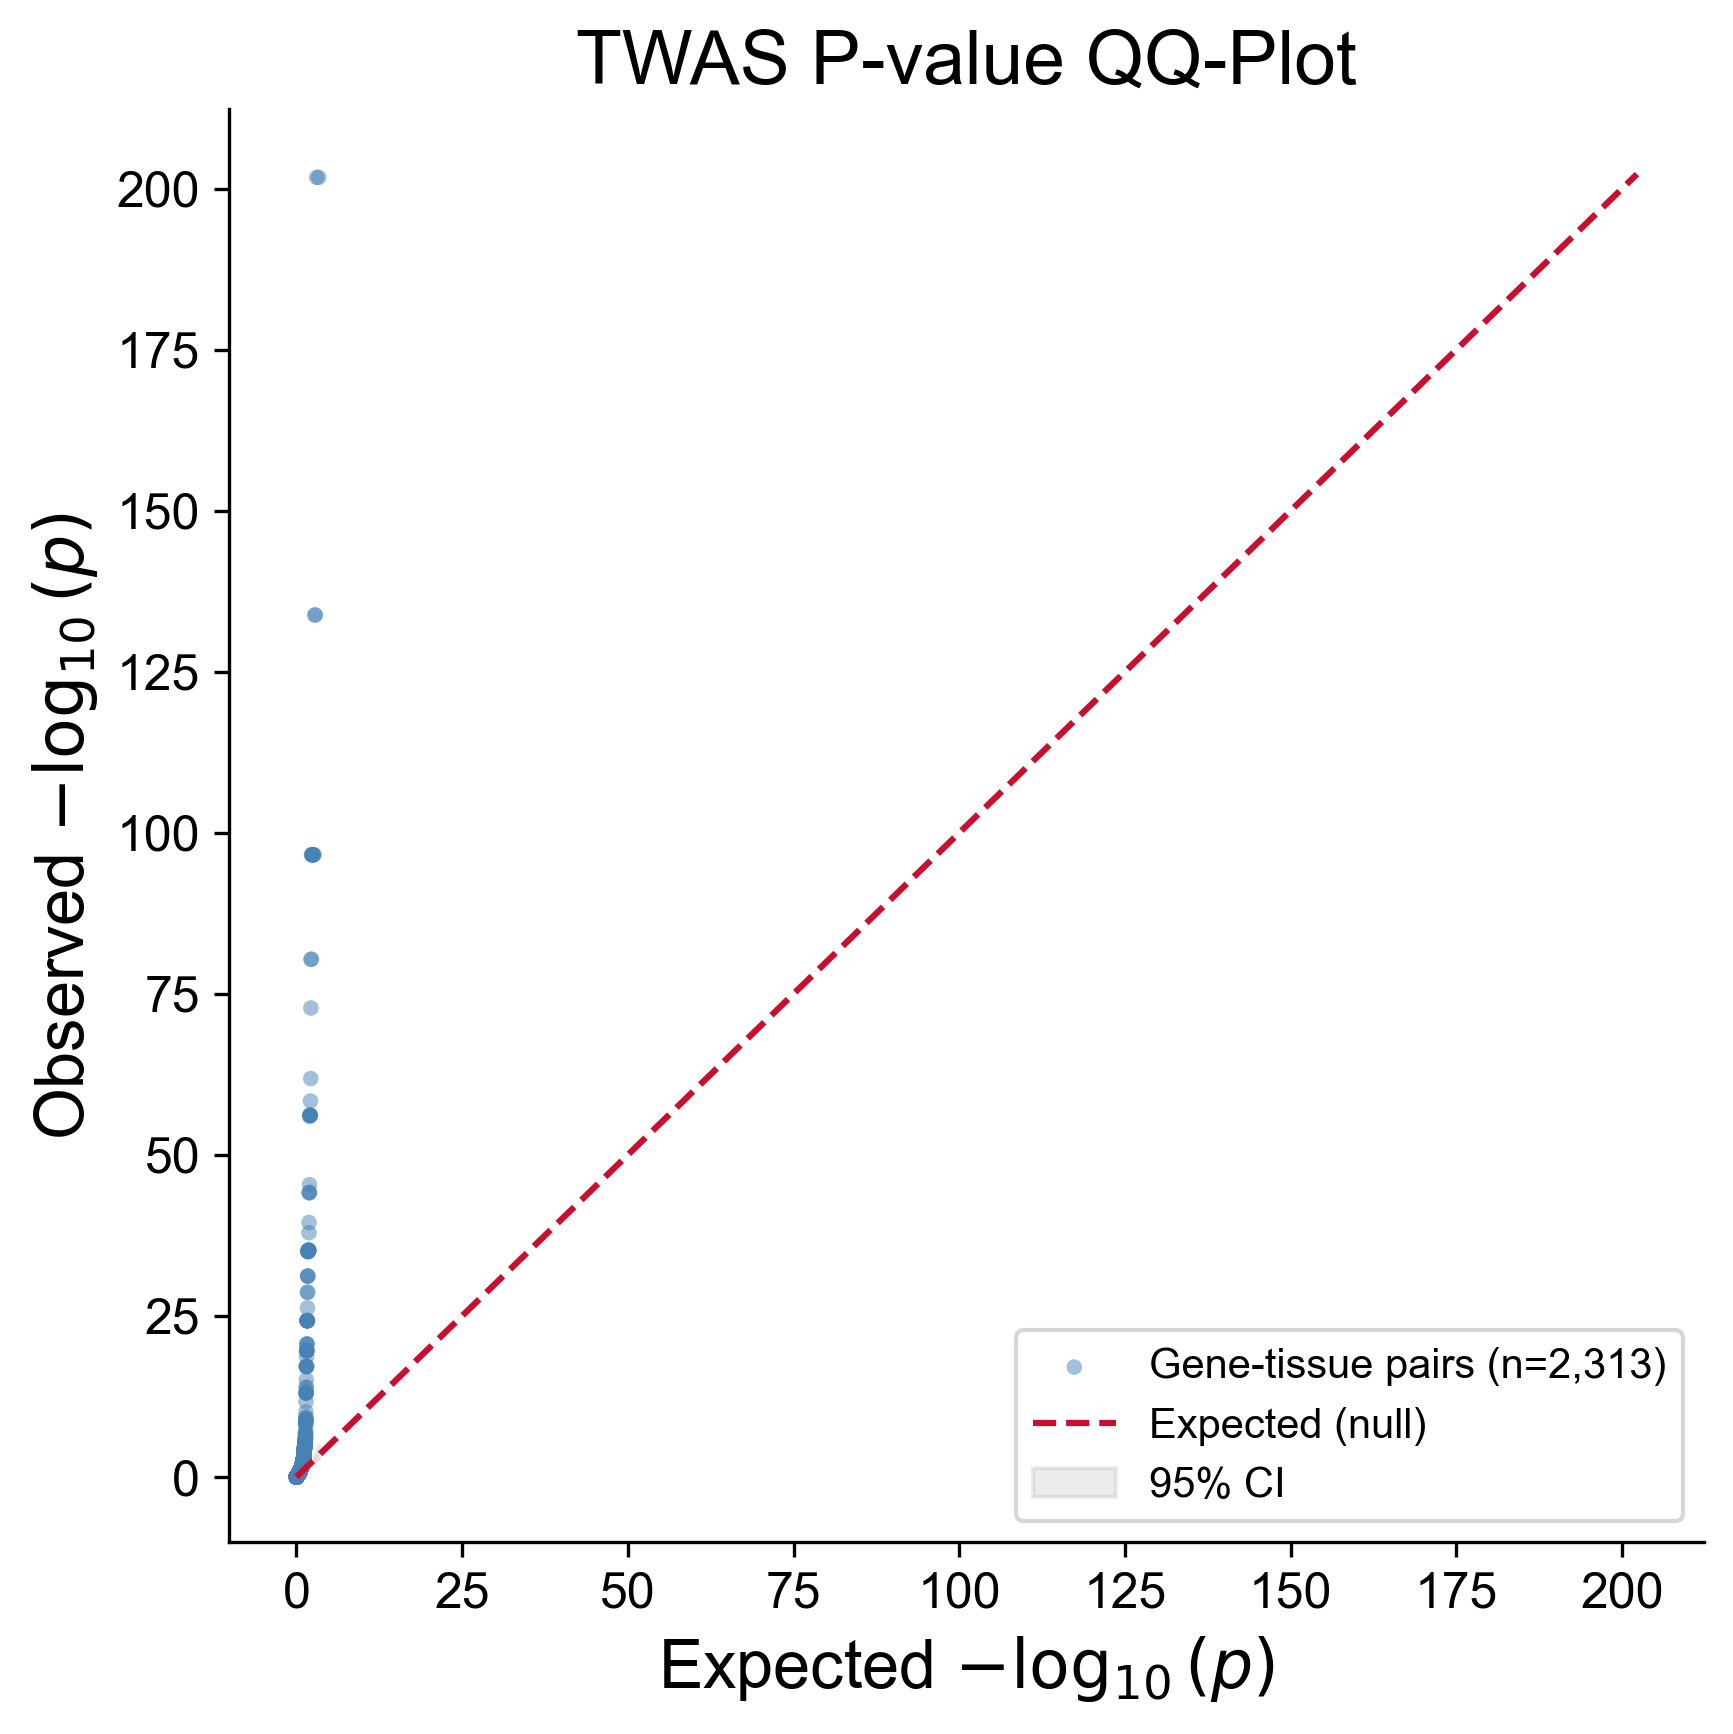
\includegraphics[width=0.55\linewidth]{figures/qqplot_twas.png}
\captionof{figure}{QQ-plot: departure from null consistent with
polygenic architecture. Grey band: 95\% CI.}
\end{center}
\end{block}

% ── Colocalization Results ───────────────────────────────────────────────────
\begin{block}{Colocalization Results}
\justifying
Of the 248 TWAS hits, Bayesian colocalization (coloc.abf) identified
\textbf{35 gene-tissue pairs (18 unique genes)} with PP4 $\geq$ 0.70,
confirming a shared causal variant between GWAS and eQTL signals.

\vskip0.3em
\begin{center}
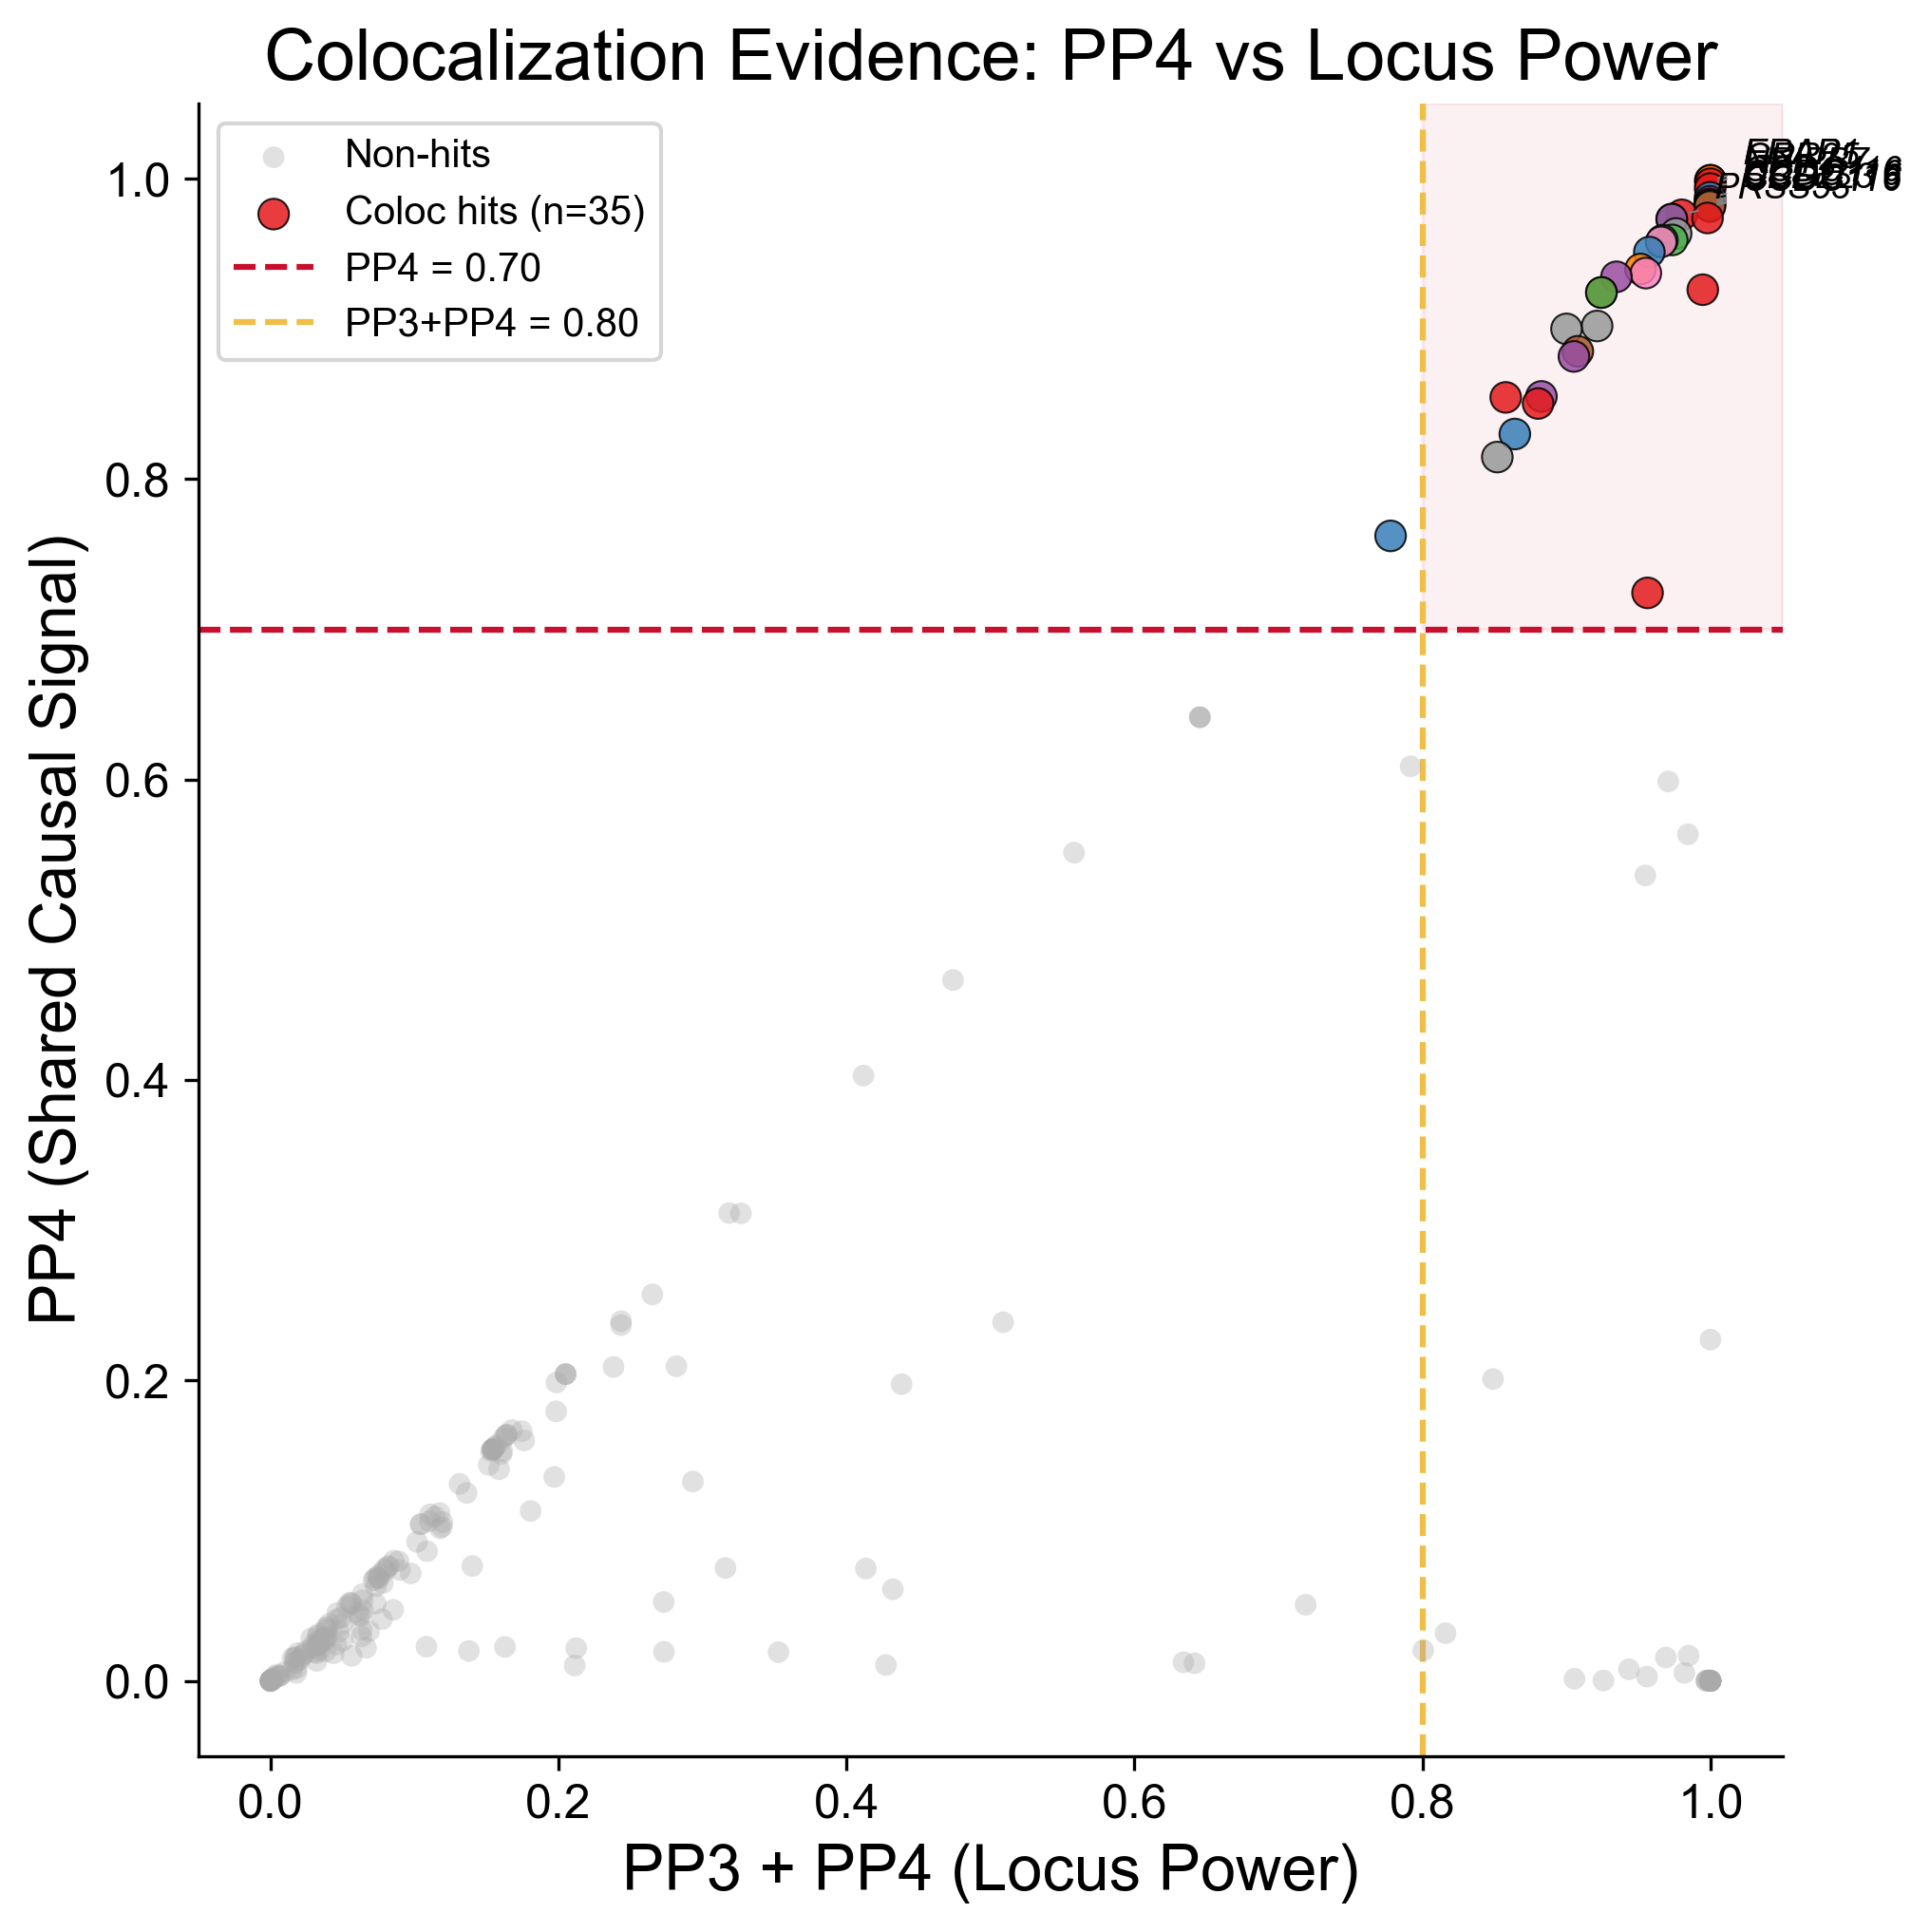
\includegraphics[width=0.60\linewidth]{figures/coloc_pp4_vs_pp3pp4.png}
\captionof{figure}{PP4 vs.\ locus power (PP3+PP4). Upper-right:
colocalization-confirmed hits.}
\end{center}
\end{block}

% ── Discussion ───────────────────────────────────────────────────────────────
\begin{block}{Discussion}
\justifying
\begin{itemize}\setlength{\itemsep}{1pt}
  \item \textit{ERAP1} (MHC-I antigen processing) is a known AS gene,
    validating our pipeline. Colocalizes in Whole Blood and Small Intestine.
  \item Novel candidates \textit{GPR25}, \textit{CCDC116}, \textit{NPIPB7}
    warrant experimental follow-up as tissue-specific drug targets.
  \item \textit{CARD9} and \textit{FAS} implicate innate immune and
    apoptotic pathways beyond HLA-B27.
  \item Colocalization reduced 248 TWAS hits to 35 confirmed pairs,
    filtering LD-driven false positives.
\end{itemize}
\end{block}

\end{column}

% ══════════════════════════════════════════════════════════════════════════════
% COLUMN 3 (right): Top Colocalized Genes, Acknowledgements & Code
% ══════════════════════════════════════════════════════════════════════════════
\begin{column}{0.32\textwidth}

% ── Top Colocalized Genes ────────────────────────────────────────────────────
\begin{block}{Top Colocalized Genes}
\begin{center}
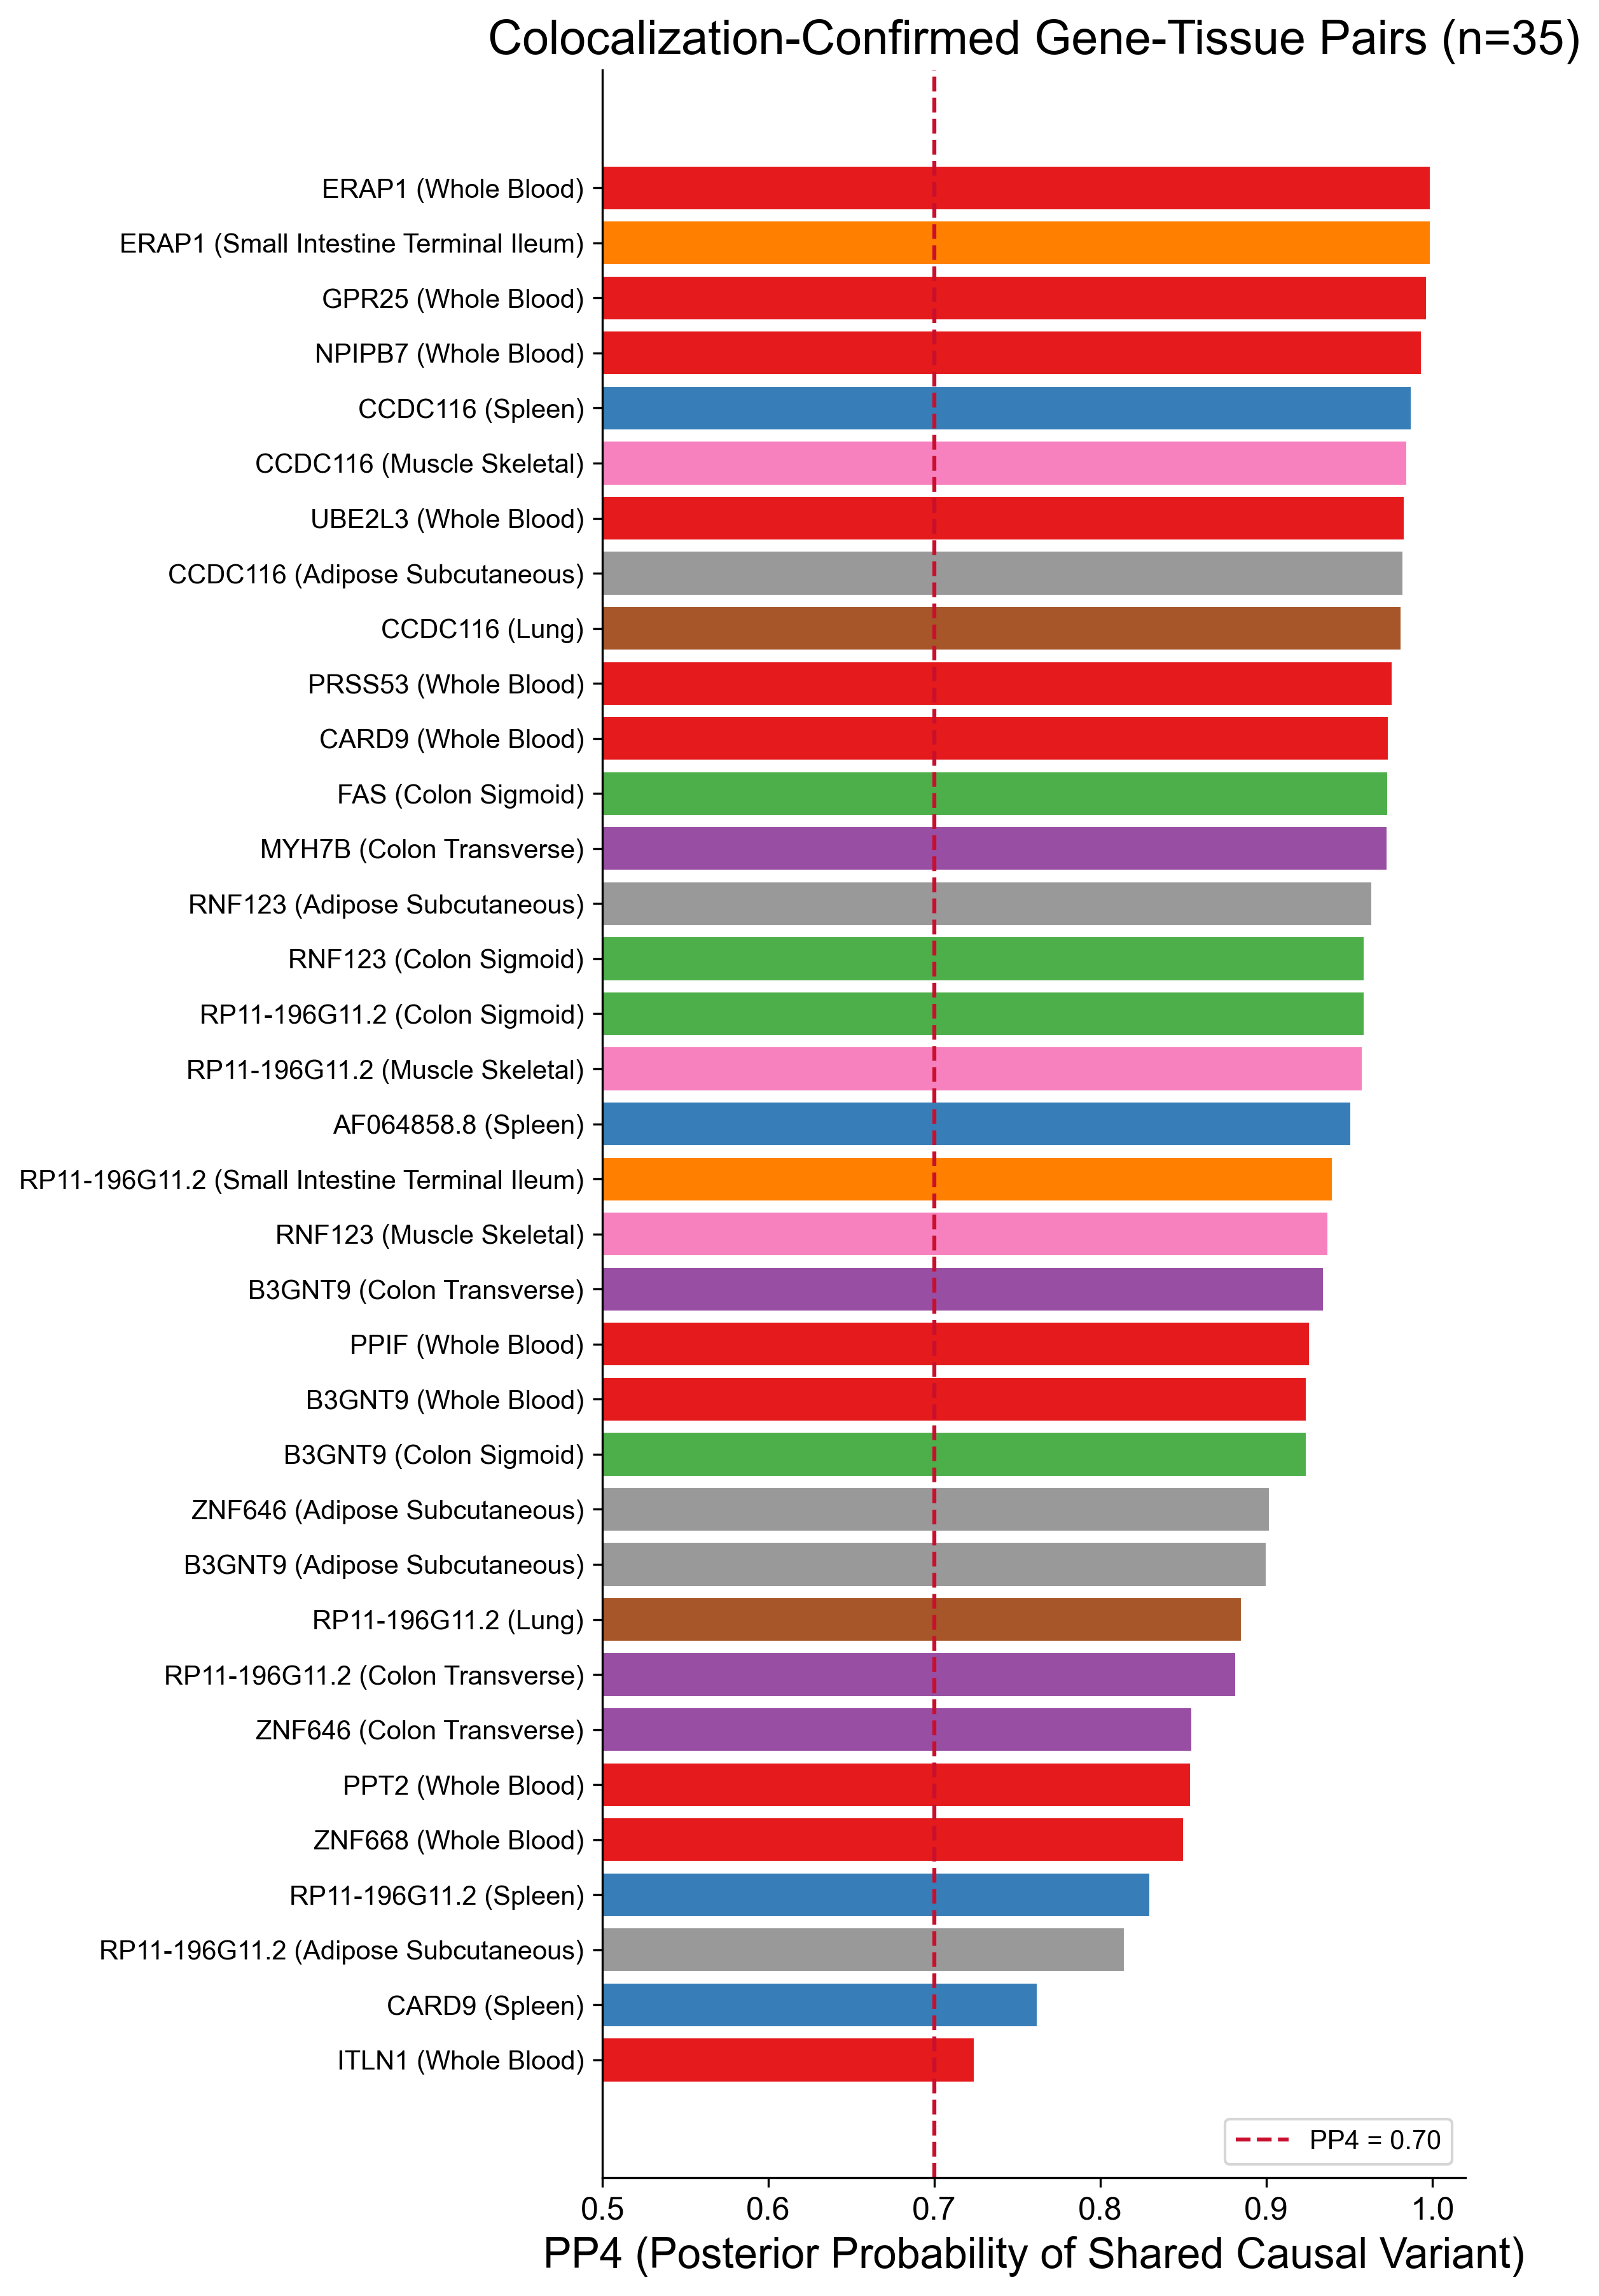
\includegraphics[width=0.92\linewidth]{figures/coloc_pp4_barplot.png}
\captionof{figure}{All 35 coloc-confirmed gene-tissue pairs ranked by PP4.
Color indicates tissue. Dashed line: PP4 = 0.70.}
\end{center}

\vskip0.3em
\footnotesize
\begin{center}
\begin{tabular}{@{}llccc@{}}
\toprule
\textbf{Gene} & \textbf{Tissue} & \textbf{PP4} & \textbf{$z$} & \textbf{FDR $p$} \\
\midrule
\textit{ERAP1}   & Whole Blood      & 0.999 & 13.28  & 2.5e-38 \\
\textit{GPR25}   & Whole Blood      & 0.997 & $-$7.03  & 6.0e-11 \\
\textit{NPIPB7}  & Whole Blood      & 0.993 & $-$5.16  & 5.9e-06 \\
\textit{CCDC116} & Spleen           & 0.988 & $-$5.16  & 5.9e-06 \\
\textit{UBE2L3}  & Whole Blood      & 0.983 & 5.32   & 2.5e-06 \\
\textit{CARD9}   & Whole Blood      & 0.974 & 4.94   & 1.7e-05 \\
\textit{FAS}     & Colon Sigmoid    & 0.973 & 4.42   & 1.9e-04 \\
\bottomrule
\end{tabular}
\end{center}
\end{block}

% ── Acknowledgements + QR ────────────────────────────────────────────────────
\begin{block}{Acknowledgements \& Code}
\begin{columns}[T,onlytextwidth]
\begin{column}{0.68\textwidth}
\footnotesize
\justifying
Thanks to \textbf{Dr.\ Ratul Chowdhury} for mentorship. GWAS data from
NHGRI-EBI GWAS Catalog (GCST005529). Expression models from GTEx
Consortium~(v8). S-PrediXcan and coloc.abf software authors.
\end{column}
\begin{column}{0.28\textwidth}
\centering
\qrcode[height=2.5cm]{https://github.com/yellepeddibk/as-twas-coloc}\\[0.2em]
\scriptsize\texttt{github.com/yellepeddibk/\\as-twas-coloc}
\end{column}
\end{columns}
\end{block}

\end{column}

\end{columns}

\end{frame}
\end{document}
